\section{Experiments with E4B}\label{sec:small}

E4B generates \ServeRatioSmallBig{} times as many tokens per second as the 31B model on the scorer's hardware
(\cref{sec:serving}), and a separate prize of the competition is reserved for the small models. Most runs of this
paper, \RunsEFour{} of \RunsTotal{}, are E4B runs. This section reports what we measured before any candidate change was tested: the first
runs on hosted notebooks, the controls of the grading path, the agreement between the workstation and the hosted
notebook, how far the unchanged baseline repeats, where it succeeds and fails, and what a run costs. The three
programmes that tried to improve the baseline follow in \cref{sec:programmes}.

\subsection{First experiments on hosted notebooks}\label{sec:small-first}

\begin{table}[t]
\centering
\footnotesize
\caption{First E4B experiments on hosted 4$\times$L4 notebooks. Time: mean seconds per job (whole job in the first block, agent phase in the others).}
\label{tab:smallfirst}
\begin{tabular}{llrrrrrrr}
\toprule
Block & Arm & Tasks & Runs & Solved & \% & 95\% interval & Time & Tool calls \\
\midrule
\texttt{pubE4-1} & \texttt{e-single} & 24 & 24 & 5 & 21 & 9--40 & 124 & 8.7 \\
\texttt{pubE4-1} & \texttt{e-wrap} & 24 & 24 & 5 & 21 & 9--40 & 108 & 10.3 \\
\texttt{pubE4-1} & \texttt{e-wrap-ad} & 24 & 24 & 5 & 21 & 9--40 & 118 & 10.5 \\
\addlinespace
\texttt{berthE4-k1} & \texttt{e-BF} & 24 & 48 & 4 & 8 & 3--20 & 70 & 9.3 \\
\texttt{berthE4-k1} & \texttt{base} & 24 & 48 & 8 & 17 & 9--30 & 79 & 11.9 \\
\addlinespace
\texttt{berthE4-k2} & \texttt{base} & 8 & 16 & 7 & 44 & 23--67 & 82 & 12.4 \\
\texttt{berthE4-k2} & \texttt{base-p} & 8 & 16 & 6 & 38 & 18--61 & 80 & 12.1 \\
\texttt{berthE4-k2} & \texttt{e-BF} & 8 & 16 & 5 & 31 & 14--56 & 58 & 8.9 \\
\texttt{berthE4-k2} & \texttt{e-BF-s} & 8 & 16 & 2 & 12 & 3--36 & 60 & 9.3 \\
\bottomrule
\end{tabular}
\end{table}


\paragraph{Development tasks.}
The first block (\texttt{pubE4-1}, \cref{tab:smallfirst}) ran three E4B arms on 24 development tasks with small
reference fixes, from three of the four repositories: a single agent (\arm{e-single}), the wrapped design of
\cref{sec:big-arms} (\arm{e-wrap}), and the wrapped design with a fine-tuned adapter on the coder (\arm{e-wrap-ad}).
Each arm solved 5 of the 24 tasks. The arms largely solved the same tasks: \SmallPubAllThree{} tasks were solved by all
three and \SmallPubUnion{} by at least one. On these 24 tasks the 31B arms \arm{BF5} and \arm{SH6} had solved
\SmallPubBigBF{} and \SmallPubBigSH{}, each in one run per task on the emulated-latency machine. The block therefore shows the size of the gap
between the two models on tasks chosen to be easy, and no difference between a single agent, a wrapped agent and an
adapter. With one run per task and five solved tasks per arm, it could only have shown a very large difference. A job
took \SmallPubWall{}~s on average and used about \SmallPubTools{} tool calls: E4B stops by itself, far inside every
limit of the scorer.

\paragraph{Berth tasks.}
The second block (\texttt{berthE4-k1}) is the first on Berth tasks: 24 tasks, two repeats, and two arms in one job
queue. \arm{e-BF} is the public single-agent prompt adapted to E4B; \arm{base} is the withheld E4B agent bundle that
we later submitted. \arm{base} solved 8 of 48 runs and \arm{e-BF} 4 of 48. By task, \arm{base} was ahead on
\KOneBaseBetter{} tasks and behind on \KOneOtherBetter{} (sign test, $p = \KOneP$); no difference was detected. We
kept \arm{base} as the baseline of every later comparison. This block is not evidence that it is the better of the
two; it is the bundle we meant to submit, and it was not behind.

The third block (\texttt{berthE4-k2}) compared four arms on eight tasks, one from each of \KTwoRepos{} repositories,
with two repeats: \arm{base}, \arm{base} with one prompt change (\arm{base-p}), \arm{e-BF}, and \arm{e-BF} with
changed sampling settings (\arm{e-BF-s}). They solved 7, 6, 5 and 2 of 16 runs. The intervals of
\cref{tab:smallfirst} overlap widely, and we drew one conclusion only: 16 runs per arm on a hosted notebook cannot
rank prompt variants of this model. The eight tasks share no task with the 24 of the second block, and the record
does not say how they were picked. \arm{base} solved 44\% of its runs on them, twice its share elsewhere, so the block
says nothing about the level of any arm. Neither \arm{base-p} nor \arm{e-BF-s} was run again.

These three blocks hold 232 runs. All later E4B experiments ran on the workstation, where the same number of runs
takes about an hour.

\subsection{Task pool and grading controls}

\begin{table}[t]
\centering
\small
\caption{Control runs of the grading path: every task graded once with its reference patch (must pass) and once with no patch (must fail).}
\label{tab:controls}
\begin{tabular}{lrr}
\toprule
Tasks and machine & Reference patch passes & Empty patch passes \\
\midrule
whole pool, workstation, no container & 580/580 & 1/580 \\
panels C and H, final runner & 200/200 & 0/200 \\
screen set S, final runner & 48/48 & 0/48 \\
case-study panel and two tasks of S, final runner & 233/233 & 0/233 \\
hosted notebook, first batch & 38/38 & 0/38 \\
hosted notebook, second batch & 87/87 & 0/209 \\
\bottomrule
\end{tabular}
\end{table}


A solved share means something only if the grading path separates a correct fix from no fix. Before any agent ran on
a task, the task was graded twice: once with its reference patch, which must pass, and once with no patch, which must
fail (\cref{tab:controls}). On the workstation, without a container, the reference patch passed on all
\PoolTasks{} tasks that loaded, from \PoolRepos{} repositories, and the empty patch passed on \PoolEmptyPass{}; that
task was removed, which leaves the \PoolValid{} tasks of \cref{sec:setting}. The controls were then repeated under the
final container runner for every panel used in this paper, and on CPU notebooks of the hosting platform for
\HostedCtrlRef{} tasks with the reference patch and \HostedCtrlEmpty{} with the empty patch. Every one of these
controls gave the expected result. \CtrlPairsMulti{} pairs of task and control were graded on more than one machine or
runner, and \CtrlPairsDisagree{} of them changed its result. The file \texttt{controls.csv} holds all \ControlRows{}
rows.

The controls test the grader, not the agent's environment. They would not show a difference in what the agent sees
while it works, for example a different Python version in its shell; \cref{sec:parity} addresses that side.

\subsection{Workstation against the hosted notebook}\label{sec:parity}

\begin{table}[t]
\centering
\small
\caption{The baseline on the same 24 Berth tasks, one run per task, on the hosted notebook and on the workstation under successive runners. Agent: mean seconds of the agent phase.}
\label{tab:parity}
\begin{tabular}{lrrr}
\toprule
Run & Solved & 95\% interval, \% & Agent \\
\midrule
hosted 4$\times$L4, repeat 1 & 4/24 & 7--36 & 79 \\
hosted 4$\times$L4, repeat 2 & 4/24 & 7--36 & 80 \\
\addlinespace
workstation, no sandbox, 8 workers & 3/24 & 4--31 & 65 \\
workstation, no sandbox, 1 worker & 5/24 & 9--40 & 63 \\
workstation, container runner, version 1 & 3/24 & 4--31 & 69 \\
workstation, container runner, version 3 & 2/24 & 2--26 & 58 \\
workstation, container runner, version 4, run a & 4/24 & 7--36 & 83 \\
workstation, container runner, version 4, run b & 3/24 & 4--31 & 70 \\
workstation, container runner, version 7 (final) & 5/24 & 9--40 & 71 \\
\bottomrule
\end{tabular}
\par\vspace{3pt}{\footnotesize\raggedright A further workstation run under runner version 2 solved 4 of 24; its result rows were not kept and it is not in the released file.\par}
\end{table}


The workstation serves the model from one GPU instead of four, runs jobs in parallel, and puts each job in a
container. Any of these could change what the agent does. \Cref{tab:parity} lists every run of the baseline on the
same 24 Berth tasks, one run per task: two repeats on the hosted notebook with four L4 GPUs, and seven runs on the
workstation as the runner changed. The first two workstation runs used no sandbox and still had the role divergence
described in \cref{sec:intro}; the others used the container runner in four of its versions.

The hosted repeats solved 4 and 4 of 24. The workstation runs solved between \ParityMin{} and \ParityMax{}, in total
\ParityWsTotal{} of \ParityWsRuns{} runs (\ParityWsPct\%) against \ParityHostedTotal{} of 48 (\ParityHostedPct\%) on
the hosted notebook. Over all 216 runs only six distinct tasks were ever solved, so the totals move because the same
few tasks come out or not, not because a runner opens or closes other tasks. The mean agent phase took 79 and 80~s on
the hosted notebook and 58 to 83~s on the workstation. Figure~\ref{fig:parity}A shows the difference of each
workstation run from the hosted share; it includes an eighth run, under runner version 2, whose rows were not kept.

What this supports is limited. With 24 tasks and one run each, the 95\% interval of 4 of 24 runs from 7\% to 36\%.
The table rules out a gross difference between the machines, such as the workstation solving half or double the
hosted share. It cannot show that a specific difference in the prompts has no effect. That question needs an
experiment with power, and \cref{sec:case} reports one.

\subsection{How far the baseline repeats}

\begin{table}[t]
\centering
\footnotesize
\caption{The unchanged baseline run again on the same tasks in separate sessions on the workstation. Range: largest minus smallest session total in percentage points. Same: tasks with the same solved count in every session. Never, always: tasks solved in no run, in every run. $r$: correlation of the per-task counts of the first and last session.}
\label{tab:repeat}
\begin{tabular}{lrllrrrrr}
\toprule
Task set & Sessions & Solved runs & \% & Range & Same & Never & Always & $r$ \\
\midrule
S (48 tasks, 2 repeats) & 3 & 19, 21, 20 & 19.8, 21.9, 20.8 & 2.1 & 39 & 34 & 5 & 0.91 \\
H (128 tasks, 4 repeats) & 2 & 103, 97 & 20.1, 18.9 & 1.2 & 99 & 83 & 10 & 0.92 \\
\bottomrule
\end{tabular}
\end{table}


\begin{figure}[t]
\centering
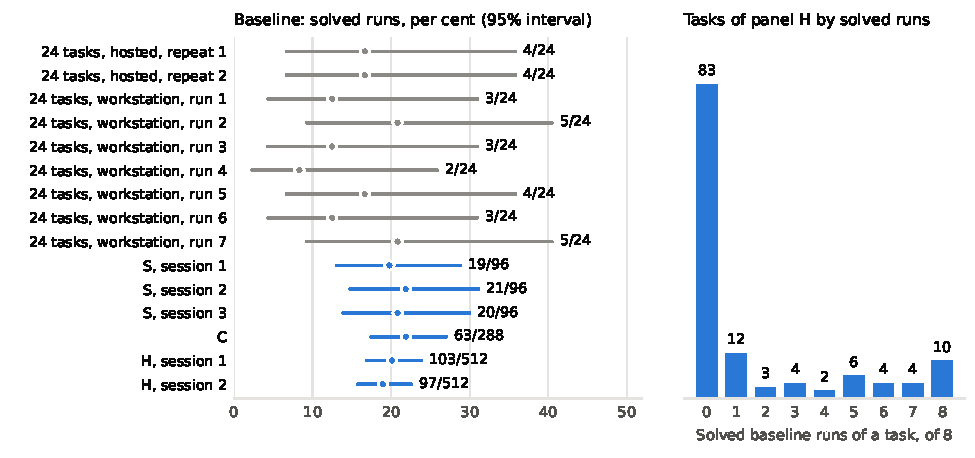
\includegraphics[width=\linewidth]{fig/repeat.pdf}
\caption{The unchanged E4B baseline on the workstation. Left: solved runs of each session on the same tasks, with
95\% intervals. Right: the 128 tasks of panel H by the number of baseline runs that solved them, of eight runs in two
sessions.}
\label{fig:repeat}
\end{figure}

Every screen and every confirmation block ran the baseline in the same job queue as the candidates. The baseline
therefore ran three times on the 48 tasks of S and twice on the 128 tasks of H, in separate sessions
(\cref{tab:repeat,fig:repeat}). On S it solved 19, 21 and 20 of 96 runs; on H,
\RepeatHFirst{} and \RepeatHSecond{} of 512. The session totals differ by at most \RepeatSRange{} points on S and by
\RepeatHDiff{} points on H.

Repeats of one task can differ. They rarely do. On H, \HNever{} of the
128 tasks (\HNeverPct\%) were solved in none of the eight baseline runs and \HAlways{} in all eight; only \HBetween{}
tasks were solved in some runs and not in others. The per-task solved counts of the two sessions correlate at 0.92.
Because so few tasks are uncertain, the run-to-run standard deviation of the total is small. Estimated from the
variation within tasks, it is \NoiseSdRuns{} runs of 512, or \NoiseSdPts{} points, for one arm and \NoiseSdDiffPts{}
points for the difference of two arms on the same tasks. The two baseline sessions differ by
\BaseSessionsDiffRuns{} runs, which is \BaseSessionsNoiseRatio{} of that standard deviation; the one pair of repeats
that we have does not contradict the estimate. The binomial formula, which treats the 512 runs as independent with one
common probability of \HBasePct\%, gives \NoiseSdBinomPts{} points; the variation within tasks accounts for
\NoiseShare\% of that variance. \Cref{sec:analysis} uses these numbers.

\subsection{Repositories}

\begin{figure}[t]
\centering
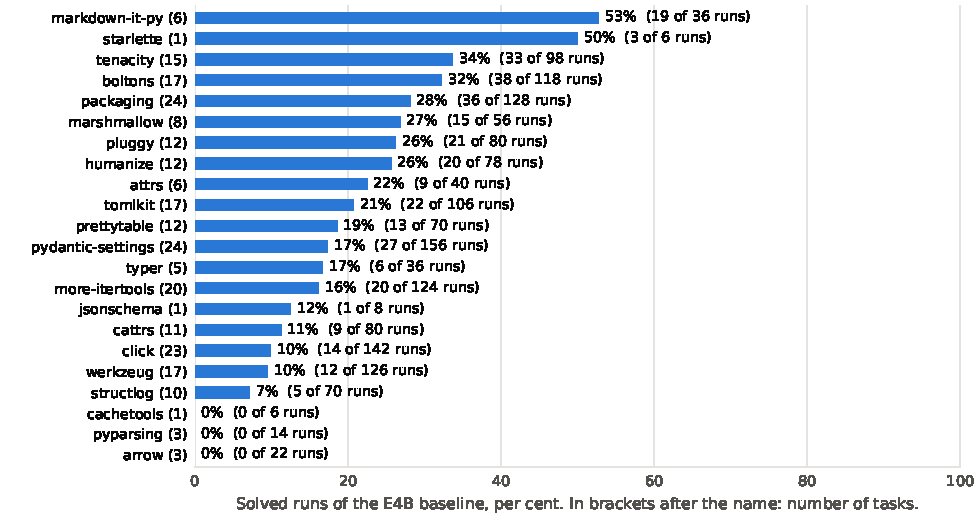
\includegraphics[width=\linewidth]{fig/repos.pdf}
\caption{Solved share of the E4B baseline by repository, over all its runs in the screen and confirmation blocks, with
95\% intervals that treat runs as independent. Numbers of tasks and runs are in \cref{tab:repos}.}
\label{fig:repos}
\end{figure}

\begin{table}[p]
\centering
\footnotesize
\caption{Solved share of the E4B baseline by repository, over every baseline run of the screen and confirmation blocks on the workstation. The interval treats runs as independent and is too narrow where few tasks carry many runs.}
\label{tab:repos}
\begin{tabular}{lrrrrr}
\toprule
Repository & Tasks & Runs & Solved & \% & 95\% interval \\
\midrule
\texttt{executablebooks/markdown-it-py} & 6 & 36 & 19 & 52.8 & 37--68 \\
\texttt{Kludex/starlette} & 1 & 6 & 3 & 50.0 & 19--81 \\
\texttt{jd/tenacity} & 15 & 98 & 33 & 33.7 & 25--43 \\
\texttt{mahmoud/boltons} & 17 & 118 & 38 & 32.2 & 24--41 \\
\texttt{pypa/packaging} & 24 & 128 & 36 & 28.1 & 21--36 \\
\texttt{marshmallow-code/marshmallow} & 8 & 56 & 15 & 26.8 & 17--40 \\
\texttt{pytest-dev/pluggy} & 12 & 80 & 21 & 26.2 & 18--37 \\
\texttt{python-humanize/humanize} & 12 & 78 & 20 & 25.6 & 17--36 \\
\texttt{python-attrs/attrs} & 6 & 40 & 9 & 22.5 & 12--38 \\
\texttt{python-poetry/tomlkit} & 17 & 106 & 22 & 20.8 & 14--29 \\
\texttt{jazzband/prettytable} & 12 & 70 & 13 & 18.6 & 11--29 \\
\texttt{pydantic/pydantic-settings} & 24 & 156 & 27 & 17.3 & 12--24 \\
\texttt{fastapi/typer} & 5 & 36 & 6 & 16.7 & 8--32 \\
\texttt{more-itertools/more-itertools} & 20 & 124 & 20 & 16.1 & 11--24 \\
\texttt{python-jsonschema/jsonschema} & 1 & 8 & 1 & 12.5 & 2--47 \\
\texttt{python-attrs/cattrs} & 11 & 80 & 9 & 11.2 & 6--20 \\
\texttt{pallets/click} & 23 & 142 & 14 & 9.9 & 6--16 \\
\texttt{pallets/werkzeug} & 17 & 126 & 12 & 9.5 & 6--16 \\
\texttt{hynek/structlog} & 10 & 70 & 5 & 7.1 & 3--16 \\
\texttt{arrow-py/arrow} & 3 & 22 & 0 & 0.0 & 0--15 \\
\texttt{pyparsing/pyparsing} & 3 & 14 & 0 & 0.0 & 0--22 \\
\texttt{tkem/cachetools} & 1 & 6 & 0 & 0.0 & 0--39 \\
\bottomrule
\end{tabular}
\end{table}


Over the screens and confirmations, the baseline ran \BaseWsRuns{} times on \BaseWsTasks{} tasks from \BaseWsRepos{}
repositories and solved \BaseWsSolved{} runs (\BaseWsPct\%). \Cref{tab:repos,fig:repos} split this by repository. The
share runs from \RepoTopPct\% in the best repository to zero in \RepoZero{} repositories; the three repositories with
the most solved runs hold \RepoTopThreeShare\% of all solved runs. The zero rows have one to three tasks each, so
they say little about those repositories. The wider pattern is firm, though: with 10 to 24 tasks each, the shares of
the larger repositories still range from 7\% to 34\%.

Two consequences follow. A change that helps in one repository can move the total visibly while doing nothing
elsewhere, which is why the pass rule of \cref{sec:compare} counts repositories and tests with repositories as
clusters. And a local total is a property of the repository mix as much as of the agent: the hidden tasks of the
scorer need not come from these repositories, and nothing here says how the baseline does on them.

\subsection{Time, tokens and failure kinds}\label{sec:cost}

\begin{table}[t]
\centering
\scriptsize\setlength{\tabcolsep}{3.1pt}
\caption{Time, tokens and endings of the agent runs by model and setting. Time: seconds per run (whole job for the development tasks, agent phase for Berth). In: prompt tokens summed over the requests of a run, in thousands. T/O, Budget, Empty: percentage of runs stopped by the time limit, stopped by the tool-call limit, and left without a patch.}
\label{tab:cost}
\begin{tabular}{p{0.2\linewidth}rrrrrrrrrrrr}
\toprule
Setting & Runs & Solved \% & Mean & Median & Solved & Unsolved & Out & In (k) & Tools & T/O & Budget & Empty \\
\midrule
31B, development tasks, emulated latency & 570 & 57.2 & 278 & 255 & 231 & 341 & 7{,}089 & 240 & 20.6 & 12.6 & 0.4 & 13.5 \\
31B, development tasks, 4$\times$L4 & 36 & 58.3 & 286 & 256 & 234 & 358 & 8{,}515 & 264 & 23.8 & 11.1 & 2.8 & 11.1 \\
31B, Berth, 4$\times$L4 & 104 & 38.5 & 226 & 212 & 165 & 265 & 7{,}495 & 196 & 19.2 & 8.7 & 0.0 & 4.8 \\
E4B, development tasks, 4$\times$L4 & 72 & 20.8 & 117 & 106 & 85 & 125 & 4{,}665 & 102 & 9.8 & 1.4 & 0.0 & 4.2 \\
E4B, Berth, 4$\times$L4 & 160 & 20.0 & 73 & 61 & 43 & 80 & 6{,}261 & 110 & 10.6 & 0.0 & 1.9 & 11.9 \\
E4B, Berth, workstation & 4{,}082 & 21.3 & 75 & 60 & 45 & 84 & 8{,}146 & 156 & 14.2 & 0.3 & 1.2 & 5.5 \\
\bottomrule
\end{tabular}
\end{table}


\begin{figure}[t]
\centering
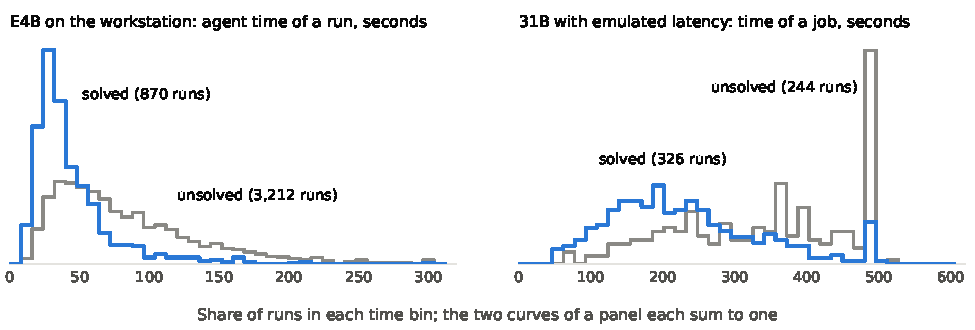
\includegraphics[width=\linewidth]{fig/time_dist.pdf}
\caption{Time of solved and unsolved runs for the two models. E4B: agent phase of the Berth runs on the workstation.
31B: whole job of the development-task runs under emulated latency.}
\label{fig:time}
\end{figure}

\Cref{tab:cost} gives time, tokens and endings for every setting in which agent runs were made, and \cref{fig:time}
the distribution of time for the two largest groups.

\paragraph{E4B is quick, and quicker when it succeeds.}
On the workstation the agent phase of an E4B run took \CostSmallMean{}~s on average: \CostSmallSolvedT{}~s when the
task was solved and \CostSmallUnsolvedT{}~s when it was not. The 31B runs on development tasks took
\CostBigMean{}~s, with \CostBigSolvedT{}~s and \CostBigUnsolvedT{}~s. The time limit ended 12.6\% of the 31B runs
and 0.3\% of the E4B runs. For the 31B model the limit is a working constraint, and the arms of \cref{sec:big} differ
mostly in how they spend it. For E4B it is not: more time would change almost nothing.

\paragraph{E4B fails by handing in a wrong fix.}
Of the \WsUnsolved{} unsolved E4B runs on the workstation, \WsUnsolvedNormalPct\% ended because the agent declared its
work finished. \WsUnsolvedWrongPct\% handed in a patch that the tests rejected, \WsUnsolvedEmptyPct\% left no patch,
and \WsUnsolvedTimeoutPct\% ran into the time limit. The typical failure is thus a wrong fix handed in after about a
minute and a half, not a run that was cut off. The three programmes of \cref{sec:programmes} accordingly changed what
the agent does within a run (its prompt, the way it edits files, an added agent step) and left the limits alone,
with one exception, an arm with a changed thinking-token limit.

\paragraph{Both models on the same tasks.}
\CommonTasks{} Berth tasks, all in S, were run with both models: with five 31B arms, the public
configurations and variants of them, on four L4 GPUs (\cref{sec:big}), and with the E4B baseline in the three screens on the workstation.
The 31B arms solved \CommonBigSolved{} of \CommonBigRuns{} runs (\CommonBigPct\%) and the E4B baseline
\CommonSmallSolved{} of \CommonSmallRuns{} (\CommonSmallPct\%). The 31B arms solved \CommonBigTasks{} of the tasks at
least once and E4B \CommonSmallTasks{}; no task was solved by E4B only. An average run took \CommonBigMean{}~s
against \CommonSmallMean{}~s, so the agent time spent per solved run is of the same order: \CommonBigPerSolved{}~s for
the 31B arms and \CommonSmallPerSolved{}~s for E4B. The comparison mixes machines and arms and covers 26 tasks; we
read it as a description, not as a test. It does say that the small model is not cheaper per solved task. It is
cheaper per attempt, and it reaches fewer tasks.

\paragraph{Totals.}
The \RunsWorkstation{} E4B runs on the workstation took \WsAgentHours{} hours of agent time in total, spread over
parallel workers, and used \WsTokensInM{} million prompt tokens and \WsTokensOutM{} million generated tokens.
